\chapter{Présentation de l'entreprise}

\section{Le groupe \asmile}

\paragraph{}
\asmile{} est une Société de Services en Ingénierie Informatique (SSII) française, dont l'activité principale repose sur le développement web et l'intégration de solutions open source\footnote{La désignation open source s'applique aux logiciels dont la licence respecte des critères précisément établis par l'Open Source Initiative, c'est-à-dire la possibilité de libre redistribution, d'accès au code source et aux travaux dérivés.~\cite{opensource}}.
\asmile{} est d'ailleurs aujourd'hui considéré comme le leader français dans le domaine.

\paragraph{}
La société a été créée en 1991 par quatre fondateurs, Jérôme Prompsy, Patrice Bertrand, Alain Arditi et Cyrille Chignardet.
\asmile{} innove alors dans le domaine des logiciels décisionnels en s'appuyant sur les méthodes de développement RAD (\textit{Rapid Application Development}).
En 1995, l'entreprise prend une nouvelle orientation du fait de la démocratisation d'Internet et des applications web.
Pionnière sur le secteur, \asmile{} se fait notamment connaître par la conception du premier site bancaire sur le web pour le Crédit Lyonnais.

\paragraph{}
En 2001, \asmile{} fait un nouveau choix stratégique en se positionnant sur les technologies open source.
En effet, en 2004, de plus en plus d'entreprises adoptent ce type de solutions qui deviennent populaires.
En 2011, \asmile{} est présent sur plusieurs gammes de produits web tels que les CMS, les portails, l'e-commerce, le décisionnel, l'ERP et l'infrastructure.
En outre, \asmile{} compte de nouveaux secteurs d'activités plus ou moins liés à l'activité du développement web : une agence média, un pôle d'exploitation, un pôle maintenance et un pôle système.

\paragraph{}
Fort de 20 ans d'expérience, \asmile{} a su se développer dans des grandes villes en métropole telles que Lyon, Bordeaux, Montpellier et Nantes.
Actuellement, le groupe continue son expansion en ouvrant d'autres agences à Aix-en-Provence, Poitiers, Grenoble et Lille.
Par ailleurs, \asmile{} manifeste aussi sa présence en Europe, avec les agences de Barcelone, Genève et Amsterdam.
Aujourd'hui, \asmile{} se développe même en dehors de l'Union européenne, grâce aux agences de Casablanca au Maroc et de Kiev en Ukraine.

L'ensemble de ces sites sont localisés sur la \reffigure{presentation:carte}.

\begin{figure}
	\centering
	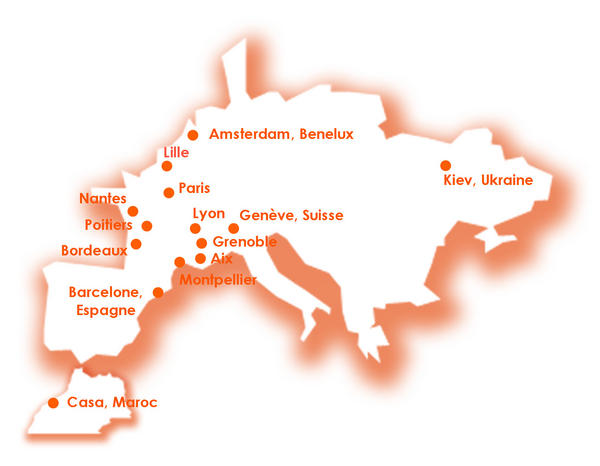
\includegraphics[width=10cm]{presentation/carte-europe-smile}
	\caption{\asmile{} en Europe}
	\label{figure:presentation:carte}
\end{figure}


\paragraph{}
Par ailleurs, l'organisation de \asmile{}, représentée en \reffigure{presentation:organigramme}, est la suivante :

\begin{itemize}
	\item en cyan, la Direction ;
	\item en beige, les BU\footnote{\textit{Business Unit}} de développement web, soit quatre unités sur Paris et quatre réparties en agences en province ;
	\item en bleu, les BU de développement européennes et offshore, qui mènent des projets locaux et des projets expertisés par Paris ;
	\item en vert, les agences métier qui regroupent les offres système, médias ainsi que les formations clients ;
	\item en violet, la BU Consulting qui gère les projets décisionnels et organisationnels.
\end{itemize}

\begin{figure}
	\centering
	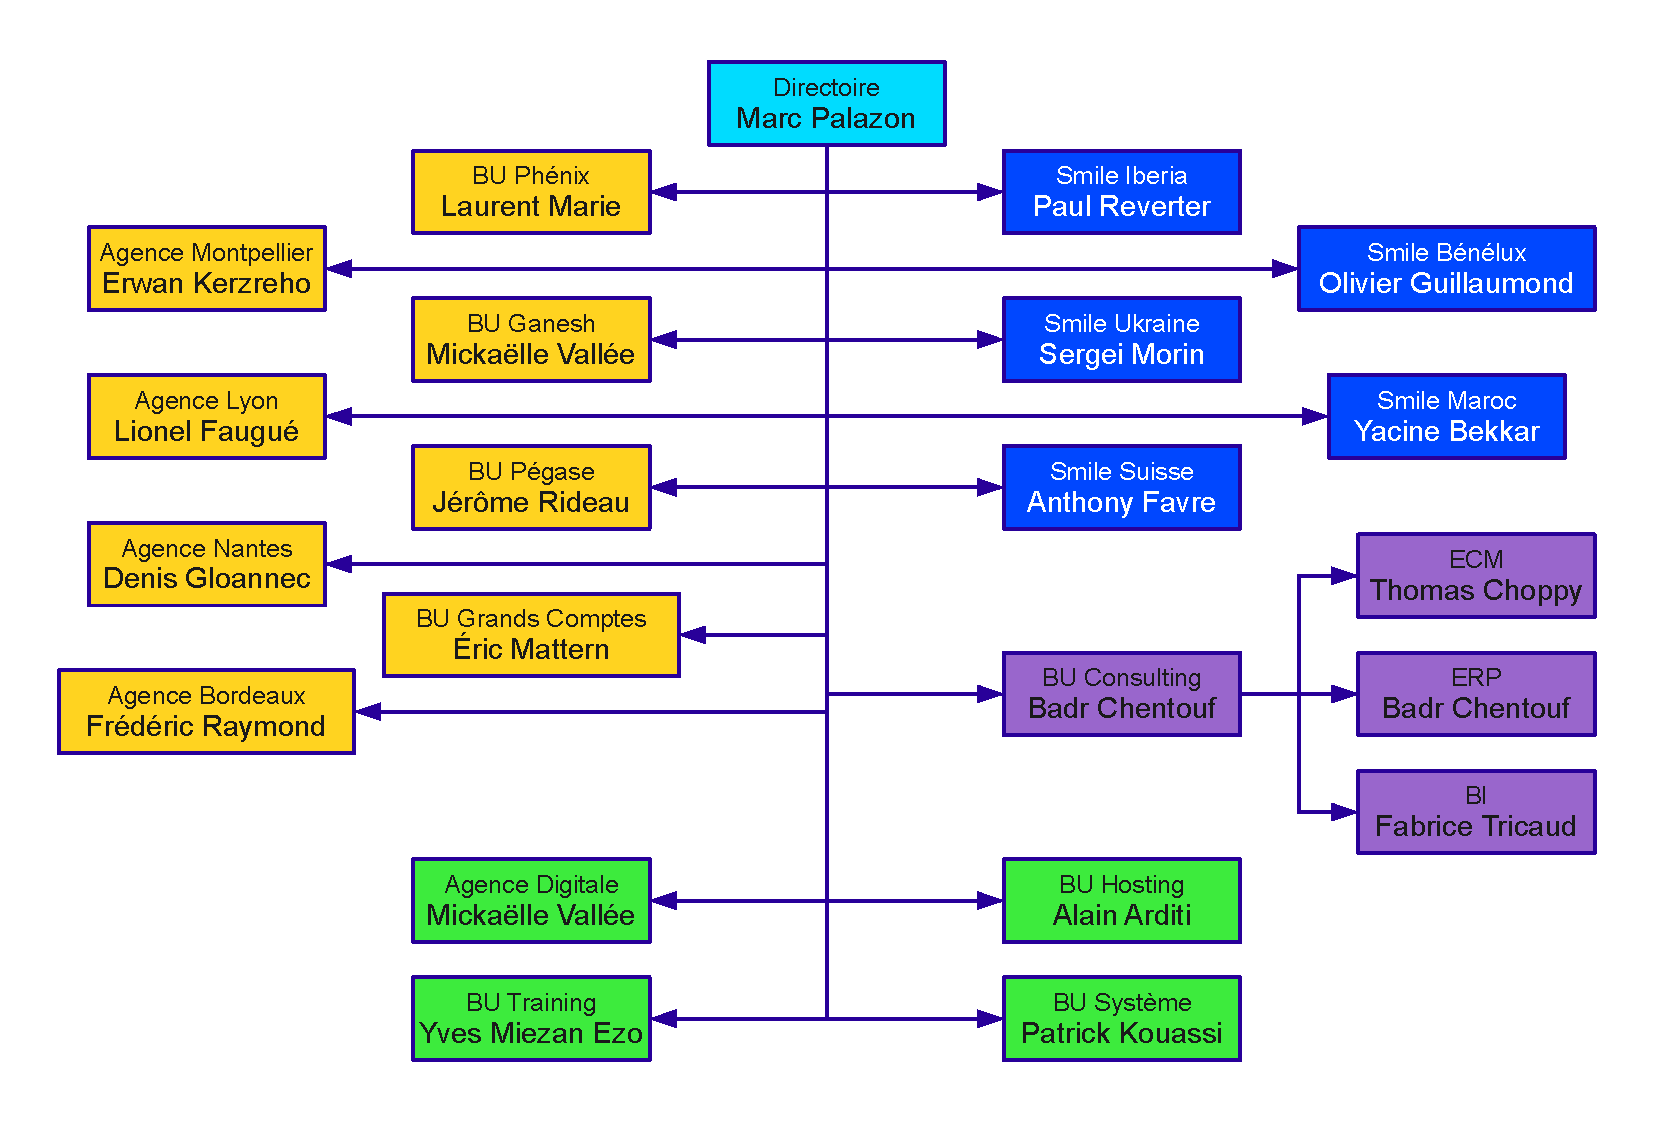
\includegraphics[width=12cm]{presentation/organigramme}
	\caption{Organigramme du groupe \asmile}
	\label{figure:presentation:organigramme}
\end{figure}


\section{Le site parisien}

\paragraph{}
Le site parisien de \asmile{} se situe à Levallois-Perret.
Elle est composée de deux bâtiments : l'un est l'ancien bâtiment de Hertford British Hospital, et l'autre un building situé à 300 mètres.
Ces bâtiments accueillent aujourd'hui plusieurs pôles de \asmile{}.

\paragraph{}
Le premier ensemble consiste en le siège social et une partie de l'administration de l'entreprise :

\begin{itemize}
	\item le bureau du Président Directeur Général, Marc Palazon ;
	\item le bureau du Directeur Général, Patrice Bertrand ;
	\item le service des Relations Humaines ;
	\item le service de la communication ;
	\item les services commerciaux ;
	\item le service financier,
	\item le système interne.
\end{itemize}

\paragraph{}
Le second regroupe des équipes métier et développement, qui sont regroupées par clients et technologies maîtrisées :

\begin{description}
	\item[la \abugan{} :] spécialiste PHP, e-commerce avec Magento, expertise CMS avec eZpublish, \atypo{}, Drupal ;
	\item[la BU Pégase :] spécialiste PHP également, e-commerce avec Magento, développement spécifique avec le framework Symfony ;
	\item[la BU Phoenix :] développements spécifiques en Java, CMS avec Jahia ;
	\item[la BU Consulting :] BI, GED, ECM, ERP ;
	\item[la BU Training :] formations ;
	\item[la \abusys{} :] c'est dans cette structure que j'ai pu travailler.
\end{description}


\section{La \abusys{}}

\paragraph{}
La \abusys{} est un pôle de prestation et de conseil dans le domaine des infrastructures système et réseau.
Le rôle de cette équipe est d'accompagner les clients dans le renouvellement et l'optimisation de leurs installations.

\paragraph{}
Pour cela, l'offre système s'articule autour de quatre solutions :

\begin{itemize}
	\item l'aide au management :
	\begin{itemize}
		\item pour les plate-formes web ;
		\item pour les infrastructures réseau ;
	\end{itemize}
	\item l'optimisation des infrastructures :
	\begin{itemize}
		\item par mutualisation des ressources grâces à des technologies de virtualisation ;
		\item par des réglages fins des outils suite à des tests de charge ;
	\end{itemize}
	\item la sécurité et gestion des accès utilisateurs :
	\begin{itemize}
		\item authentification ;
		\item VPN ;
		\item firewalls ;
	\end{itemize}
	\item l'étude de solutions haute disponibilité ;
	\item la migration vers des solutions open source :
	\begin{itemize}
		\item re-packaging de distributions Linux ;
		\item solutions de messageries et groupeware ;
		\item VoIP ;
		\item plate-formes d'intégration continue\ldots
	\end{itemize}
\end{itemize}

\paragraph{}
Aussi, la \abusys{} propose une offre interne de support projet pour les autres BU et agences de
\asmile{} :

\begin{itemize}
	\item le déploiement d'environnements de recette pour les projets de développement ;
	\item l'intégration des infrastructures évoluées, comme la haute disponibilité par exemple ;
	\item le soutien aux projets au niveau système.
\end{itemize}

\paragraph{}
Finalement, pour chaque besoin de l'entreprise la \abusys{} peut proposer une solution open source adaptée.
L'offre système est illustrée en \reffigure{presentation:offre-sys}.

\begin{figure}
	\centering
	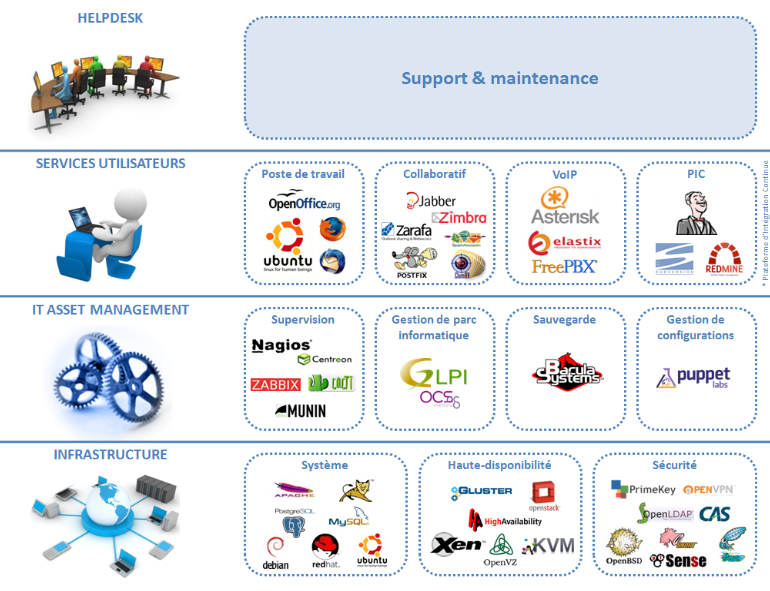
\includegraphics[width=12cm]{presentation/offre-sys}
	\caption{L'offre de la \abusys}
	\label{figure:presentation:offre-sys}
\end{figure}

